\usepackage[
    locale=DE 
    separate-uncertainty=true 
    per-mode=symblo-or-fraction
]{siunitx}


\section{Auswertung}
\label{sec:Auswertung}

\subsection{Messdaten}
%Tabelle mit Messdaten in SI

\begin{table}
    \centering
    \caption{Messdaten}
    \label{tab:Messdaten}
    \begin{tabular}{S S S S S S}
        \toprule
        {$t [s]$} & {$T1 [K]$} & {$p1 [Pa]$} & {$T2 [K]$} & {$p2 [Pa]$} & {$N [W]$} \\
        \midrule
        0.00   &      294.85  &   500000.00  &      294.85  &   510000.00  &      120.00 \\
        60.00  &      296.15  &   600000.00  &      294.85  &   420000.00  &      120.00\\
       120.00  &      297.45  &   650000.00  &      294.75  &   440000.00  &      120.00\\
       180.00  &      298.45  &   700000.00  &      294.65  &   450000.00  &      120.00\\
       240.00  &      299.55  &   700000.00  &      293.95  &   450000.00  &      120.00\\
       300.00  &      300.65  &   700000.00  &      293.25  &   440000.00  &      120.00\\
       360.00  &      301.95  &   750000.00  &      292.35  &   430000.00  &      120.00\\
       420.00  &      302.85  &   750000.00  &      291.65  &   420000.00  &      120.00\\
       480.00  &      304.05  &   800000.00  &      290.85  &   420000.00  &      120.00\\
       540.00  &      305.05  &   800000.00  &      290.05  &   400000.00  &      120.00\\
       600.00  &      306.05  &   800000.00  &      289.35  &   400000.00  &      120.00\\
       660.00  &      307.05  &   850000.00  &      288.65  &   390000.00  &      120.00\\
       720.00  &      307.95  &   850000.00  &      288.05  &   380000.00  &      120.00\\
       780.00  &      308.85  &   900000.00  &      287.35  &   380000.00  &      120.00\\
       840.00  &      309.85  &   900000.00  &      286.75  &   370000.00  &      120.00\\
       900.00  &      310.75  &   900000.00  &      286.15  &   360000.00  &      120.00\\
       960.00  &      311.55  &   950000.00  &      285.55  &   360000.00  &      120.00\\
      1020.00  &      312.35  &   950000.00  &      284.85  &   360000.00  &      120.00\\
      1080.00  &      313.15  &  1000000.00  &      284.45  &   350000.00  &      120.00\\
      1140.00  &      313.85  &  1000000.00  &      284.05  &   350000.00  &      120.00\\
      1200.00  &      314.55  &  1000000.00  &      283.55  &   340000.00  &      120.00\\
      1260.00  &      315.35  &  1000000.00  &      283.05  &   340000.00  &      120.00\\
      1320.00  &      316.05  &  1050000.00  &      282.65  &   340000.00  &      120.00\\
      1380.00  &      316.75  &  1050000.00  &      282.25  &   340000.00  &      120.00\\
      1440.00  &      317.45  &  1100000.00  &      281.85  &   340000.00  &      120.00\\
      1500.00  &      318.05  &  1100000.00  &      281.45  &   340000.00  &      120.00\\
      1560.00  &      318.65  &  1100000.00  &      281.15  &   330000.00  &      120.00\\
      1620.00  &      319.25  &  1100000.00  &      280.85  &   320000.00  &      122.00\\
      1680.00  &      319.85  &  1150000.00  &      280.55  &   320000.00  &      122.00\\
      1740.00  &      320.45  &  1150000.00  &      280.25  &   320000.00  &      122.00\\
      1800.00  &      320.95  &  1175000.00  &      279.95  &   320000.00  &      122.00\\
      1860.00  &      321.55  &  1200000.00  &      278.75  &   320000.00  &      122.00\\
      1920.00  &      322.05  &  1200000.00  &      277.45  &   320000.00  &      122.00\\
      1980.00  &      322.55  &  1200000.00  &      276.55  &   320000.00  &      122.00\\
      2040.00  &      323.05  &  1200000.00  &      276.15  &   320000.00  &      122.00\\
      2100.00  &      323.45  &  1200000.00  &      276.05  &   320000.00  &      122.00\\   
        \bottomrule
    \end{tabular}
\end{table}

\subsection{Temperaturverläufe}
%Aufgabenteil a)
\subsection{Temperaturmessung}
Im folgenden Diagramm werden die Verläufe der Temperaturen T1 und T2 in Abhängigkeit der Zeit aufgetragen.
Alle Werte wurden in SI-Einheiten konvertiert.
\begin{figure}
  \centering
  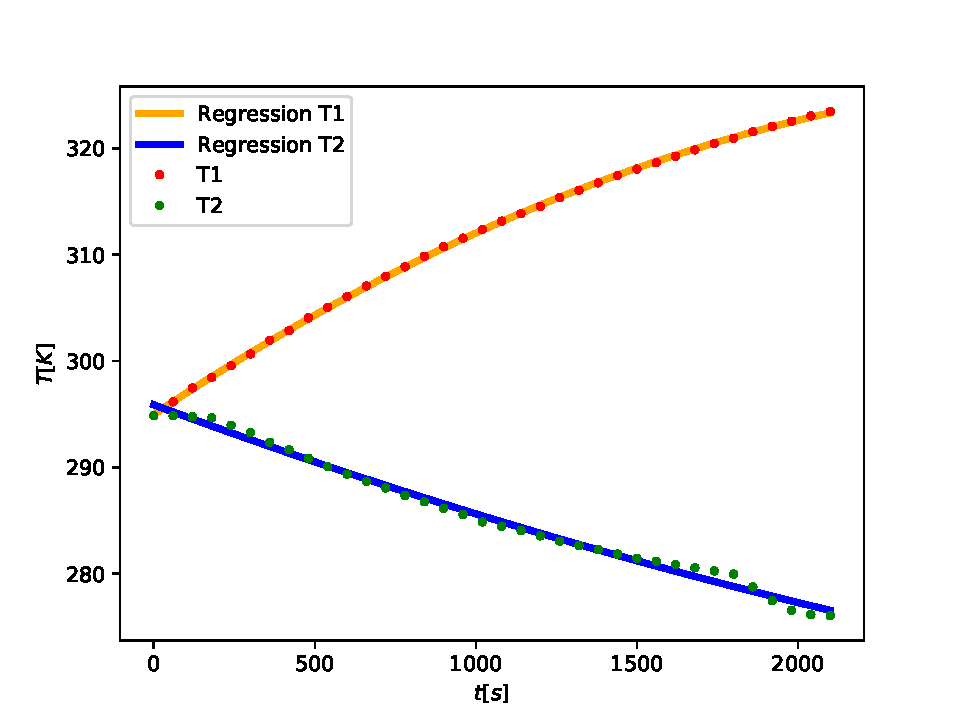
\includegraphics[scale = 0.75]{Temperaturverlaeufe.pdf}
  \caption{Die beiden Temperaturverläufe der Reservoire 1 und 2.}
  \label{fig:TemperaturverlaufA}
\end{figure}

%Aufgabenteil b)
\subsection{Bestimmung der Näherungsfunktion}
Die nicht-linearen Ausgleichsrechnungen sind ebenfalls in \ref{fig:TemperaturverlaufA} skizziert. Der gewählte Ansatz ist
\begin{equation}
  T(t) = \symup{A} \cdot t^2 + \symup{B} \cdot t + \symup{C}.
  \label{eq:Regressionsgleichung}
\end{equation}
\begin{table}
  \centering
  \caption{Parameter der nicht-linearen Ausgleichsrechnung}
  \label{tab:regression1}
  \sisetup{table-format=1.5}
  \begin{tabular}{c S S S S S S}
    \toprule
     {$T$} & {$A [K/s^2]$} & {$\increment A [K/s^2]$} & {$B [K/s]$} & {$\increment B [K/s]$} & {$C [K]$} & {$\increment C [K]$} \\
    \midrule
    {$T_\text{1}$} & 3.2249e-6 &  $\pm$4.1934e-8 &  0.02027984 & $\pm$9.11047e-5 & 294.97008 & $\pm$0.04134 \\
    {$T_\text{2}$} & 0.9550e-6 &  $\pm$26.711e-8 & -0.01120872 & $\pm$58.0316e-5 & 295.87019 & $\pm$0.26336 \\
    
      \bottomrule
  \end{tabular}
\end{table}

%Aufgabenteil c)
\subsection{Bestimmung der Differentailquotienten}
Die Differentailquotienten der Regressionen berechnet man durch einfaches Ableiten der Gleichung \eqref{eq:Regressionsgleichung}.
Nach den Ableitungsregeln ergibt sich:
\begin{equation}
    T'(t) = 2\symup{A} \cdot t + \symup{B}
    \label{eq:Regressionableitung}
  \end{equation}
  Nun werden konkrete Werte für 4 verschiedene Temperaturen berechnet werden. Diese sind in unserem Fall die Temperaturen bei 
  den Zeiten $60s, 660s, 1 260s, 1 860s$.
  \begin{table}
    \centering
    \caption{Differentailquotienten}
    \label{tab:Differentailquotienten}
    \sisetup{table-format=1.5}
    \begin{tabular}{c S S S S S S}
      \toprule
       {$t [s]$} & {$T_{1}'(t) [K/s]$} & {$\increment T_{1}'(t) [K/s]$} & {$T_{2}'(t) [K/s]$} & {$\increment T_{2}'(t) [K/s]$} \\
      \midrule
      60 & 0.02027 & 9.11047e-5 & 0.01121 & 5.80316e-4 
      660 & 0.02020 & 9.11047e-5 & 0.01118 & 5.80345e-4 
      1 260 & 0.020144 & 9.11216e-5 & 0.01117 & 5.80424e-4 
      1 860 & 0.020079 & 9.11417e-5 & 0.01115 & 5.80552e-4
      
        \bottomrule
    \end{tabular}
  \end{table}

\subsection{Bestimmung der Güteziffer}
Mithilfe der Differentailquotienten soll mit \eqref{realegütezifffer3} die reale Güteziffer berechnet werden. Zudem soll diese mit der
idealen Güteziffer verglichen werden, die mit \eqref{idealegüteziffer} berechnet wird. 
Die Abweichung p der Beiden Werte in Prozent wird berechnet mit:
\begin{equation}
  p=\frac{v_{id}-v_{real}}{v_{id}} \cdot 100
\end{equation}
Die Berechnung bei den vier oben beschriebenen
Zeitpunkten ergibt: 
\begin{table}
  \centering
  \caption{Güteziffern}
  \label{tab:güteziffer}
  \sisetup{table-format=1.5}
  \begin{tabular}{S S S S S S S S S S S}
    \toprule
     {$t [s]$} & {$v_{real1}$} & {$\increment v_{real1}$}& {$v_{real2}$} & {$\increment v_{real2}$} & {$v_{id1}$} & {$v_id2$} & {$p_1$} & {$\increment p_1$} & {$p_2$} & {$\increment p_1$} \\
    \midrule
    60 & 2.95349 & 0.01327 & 1.63264 & 0.08454 & 227 & 226 & 98.70351 & 0.00583 & 99.28016 & 0.03727 \\
    660 & 2.94409 & 0.01327 & 1.62986 & 0.08454 & 16 & 15 & 82.35746 & 0.07954 & 89.61044 & 0.53894 \\
    1 260 & 2.93470 & 0.01327 & 1.62707 & 0.08456 & 9 & 8 & 69.94106 & 0.13597 & 69.94105 & 0.96492 \\
    1 860 & 2.87735 & 0.01306 & 1.59767 & 0.08319 & 7 & 6 & 61.70096 & 0.17384 & 75.46897 & 1.27773 \\
      \bottomrule
  \end{tabular}
\end{table}

Es fällt auf, dass die Abweichung der realen Güteziffer von dem idealen Wert stark abweicht. 
Mögliche Gründe für diese Abweichung werden in \ref{sec:Diskussion} angegeben.

\subsection{Bestimmung des Massendurchsatzes}
Die Berechnung des Massendurchsatzes erfolgt mit \eqref{eqn:massendurchsatz2}. Dafür muss aber zuerst die 
Verdampfungswärme L bestimmt werden. 
\\
Aus V203-"Verdampfungswärme" ist folgender Zusammenhang zwischen dem Druck p, der Temperatur T, und L bekannt:
\begin{equation}
  ln(p/p0)=\frac{-L}{R \cdot T}
\end{equation}
R entspricht hierbei der universellen Gaskonstante und p_0 entspricht der Umgebungsdruck.
Wählt man nun $x=1/T$ und $y=ln(p-p_0)$, dann erhält man die lineare Gleichung:
\begin{equation}
  y=-\frac{L}{R}*x+c \label{Dampfdruckgleichung}
\end{equation}
Trägt man die Messwerte in ein Koordinaten System ein und setzt wie oben beschrieben $x=1/T$ und $y=ln(p-p_0)$,
wird dieser Zusammenhang gut ersichtlich.
\begin{figure}
  \centering
  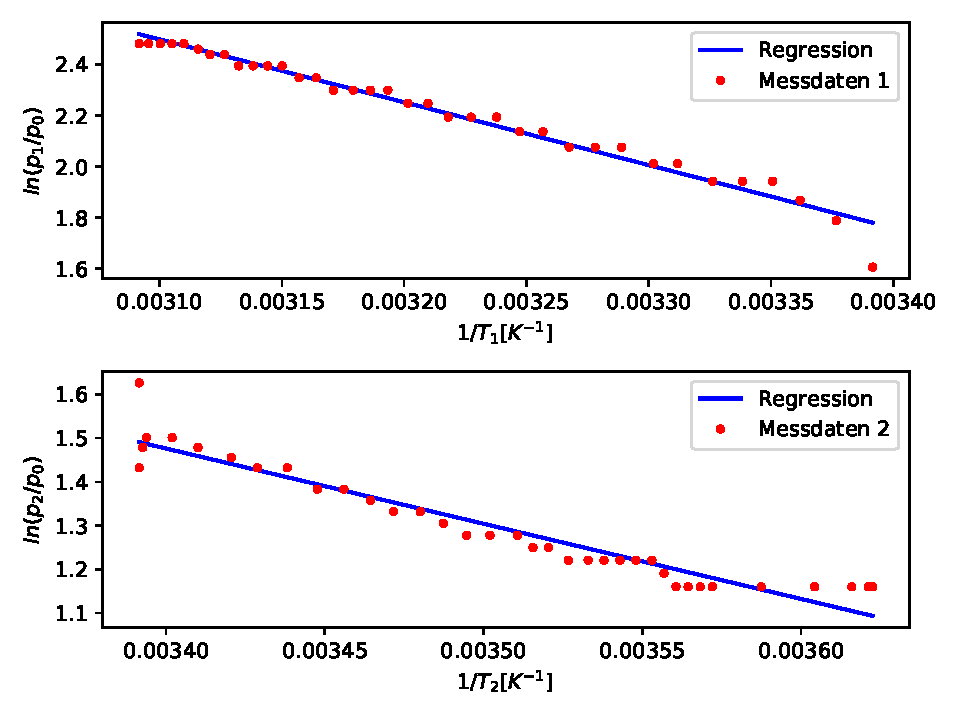
\includegraphics[scale = 0.75]{Druckverlaeufe.pdf}
  \caption{Dampfdruckkurve}
  \label{fig:Dampfdruckkurve}
\end{figure}
Die eingezeichnete Regression hat nun genau die Funktionsgleichung \eqref{Dampfdruckgleichung}. Die Steigung der 
Gerade ist demnach $m=-L/R$. L erhält also durch $L=-m*R$. Durch Einsetzen folgt:
\\
L=\SI{14299.459+/-734.742}{\joule\second\kelvin\per\mole}
\\
Mit \eqref{eqn:massendurchsatz2} kann man jetzt für die vier verschiedenen Zeiten den Massendurchsatz errechnen:
\begin{table}
  \centering
  \caption{Massendurchsatz}
  \label{tab:massendurchsatz}
  \sisetup{table-format=1.5}
  \begin{tabular}{S S S S S}
    \toprule
    {$t [s]$} & {$\frac{dm}{dt} [mol/s]$} & {$\increment\frac{dm}{dt}[mol/s]$} & {$\frac{dm}{dt} [g/s]$} & {$\increment\frac{dm}{dt}[g/s]$} \\
    \midrule
    60 & 0.01370 & 0.00100 & 1.65659 & 0.12084 \\
    660 & 0.01365 & 0.00100 & 1.65377 & 0.12075 \\
    1 260 & 0.01365 & 0.00100 & 1.65095 & 0.12065 \\
    1 860 & 0.01363 & 0.00100 & 1.64812 & 0.12057 \\
    \bottomrule
  \end{tabular}
\end{table}
Der Massendurchsatz wird in \ref{tab:massendurchsatz} sowohl in $\si{\mole\per\second}$, als auch in $\si{\gram\per\second}$ angegeben.
Man erreicht die Umrechnung mit:
\begin{equation}
  m=M\cdot n
\end{equation}
Hierbei ist $M$ die Molmasse des Gases Dichlordifluormethan $M_{CCl_{2}F_{2}}=\SIlist{120.9}{\kilogram\per\mole}$.

\subsection{Bestimmung der mechanischen Kompressorleistung}
Die mechanische Kompressorleistung $N_{mech}$ wird mit \eqref{eqn:leistungkompressor2} berechnet.
Dabei gilt:
\begin{equation}
  \frac{\Delta V_a}{\Delta t}=\frac{1}{\rho}\frac{dm}{dt} \label{Volumenänderung}
\end{equation}
Das $\rho$ hierbei die Dichte des Gases in Abhängigkeit der Temperatur und des Drucks.
Die Dichte kann man nun mit dem idealen Gasgesetz
\begin{equation}
  pV=nRT \Leftrightarrow \frac{pV}{T}=nR
\end{equation}
berechnen. Da die Stoffmenge $n$ des Gases immer konstant ist, da kein Gas entweicht oder zugeführt wird, und auch
$R$ eine Konstante ist, ist die ganze Rechte Seite konstant. Diese Seite ist für die Temperatur $T_2$, den Druck $p_2$ und das
Volumen $V_2$ gleich den Werten, bei denen die Dichte $\rho_0=\SI{5.514}{\gram\liter}$ des Gases gemessen wurde. Diese lauten
$p_0=\SI{10^5}{\pascal}$ und $T_0=\SI{273.15}{kelvin}$.
\begin{equation}
  \frac{p_2V_2}{T_2}=\frac{p_0V_0}{T_0} \Leftrightarrow \frac{p_2m}{\rho_2T_2}=\frac{p_0m}{\rho_0T_0}
\end{equation}
Da die auch die Masse des Gases konstant ist, kann diese herraus gekürzt werden.
Umstellen nach $\rho_2=\rho$ ergibt:
\begin{equation}
  \rho=\frac{\rho_0T_0p_1}{T_2p_0} \label{rho}
\end{equation}
\\
Mit \eqref{rho} und \eqref{Volumenänderung} kann \eqref{eqn:leistungkompressor2} geschrieben werden als:
\begin{equation}
  N_\text{mech} = \frac{1}{\kappa - 1}  \left(p_\text{b} \sqrt[\kappa]{\frac{p_\text{a}}{p_\text{b}}} - p_\text{a} \right)
  \frac{T_2p_0}{\rho_0T_0p_a}\frac{dm}{dt}
\end{equation}
Die mechanische Leistung des Kompressors ist nach Einsetzen der vier ausgewählten Zeiten:
\begin{table}
  \centering
  \caption{mechanische Kompressorleistung}
  \label{tab:kompressorleistung}
  \sisetup{table-format=1.5}
\begin{tabular}{S S S S S}
  \toprule
  {$t [s]$} & {$N_\text{mech} [W]$} & {$\increment N_\text{mech} [W]$} & {$\rho [kg/m^3]$} & {$\increment\rho [kg/m^3]$} \\
  \midrule
  60 & 18.02604 & 0.92977 & 30.53529 & 0.01356\\
  660 & 37.45139 & 1.93178 & 44.18748 & 0.01530\\
  1 260 & 49.78378 & 2.56797 & 53.01378 & 0.01873\\
  1 860 & 59.01109 & 3.04402 & 64.59788 & 0.02317\\
  \bottomrule
\end{tabular}
\end{table}